\Large
The Pandas library provides the user with two main data structures: one-dimensional Series
and two-dimensional DataFrame.
To interpret the program with Pandas over the abstract domain, we define the abstract lattice.
The Figures~\ref{fig:hierarchy}~and~\ref{fig:upper_part} show how the abstract lattice is defined.

\begin{tikzfigure}[Lower part of the Lattice]
    \label{fig:hierarchy}
    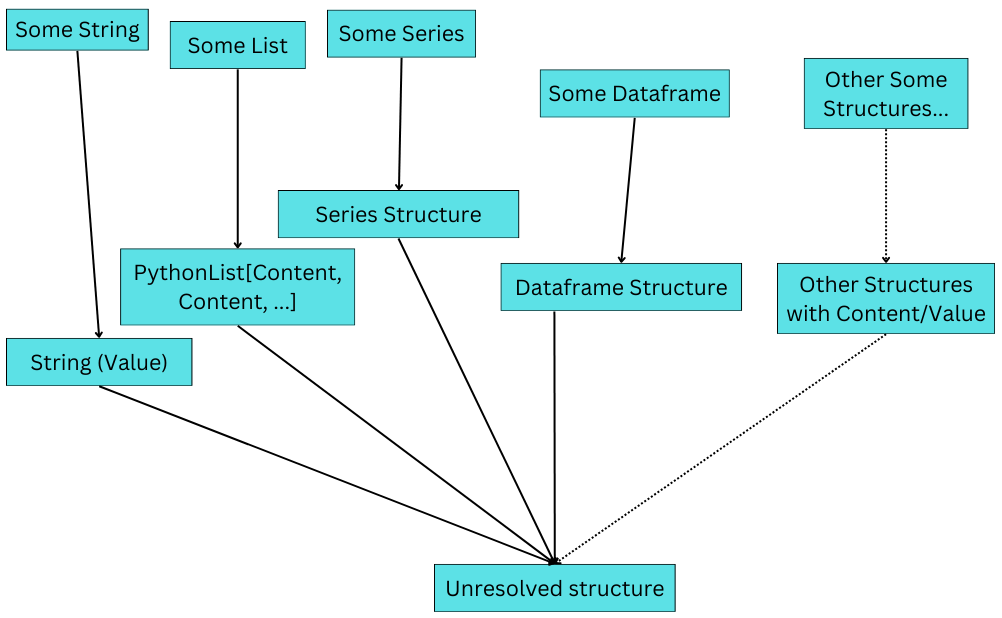
\includegraphics[scale=0.7]{poster/img/hier}
\end{tikzfigure}

\begin{tikzfigure}[Upper part of the Lattice]
    \label{fig:upper_part}
    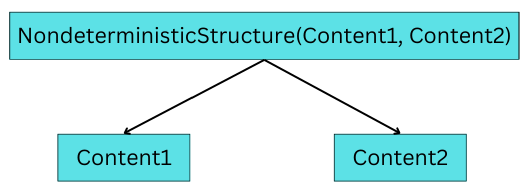
\includegraphics[scale=0.7]{poster/img/nondeterm}
\end{tikzfigure}

There is the UnresolvedStructure at the bottom of the hierarchy, representing a value that we were not
able to derive (due to error in execution).
And there is a NondeterministicStructure as a supremum for each pair representing uncertainty between two options.
The uncertainty usually occurs in the uncertain if-statement.
